% https://gitlab.com/tikz-goodies/tikz-goodies/-/blob/master/drawstack/stack-example.tex
\documentclass[tikz,border=10pt]{standalone}

\usepackage{drawstack}

% Use this instead if you don't want colors.
% \usepackage[nocolor]{drawstack}

\title{{\tt drawstack.sty}: Draw execution stack easily in LaTeX}
\author{Matthieu Moy}

\begin{document}
	
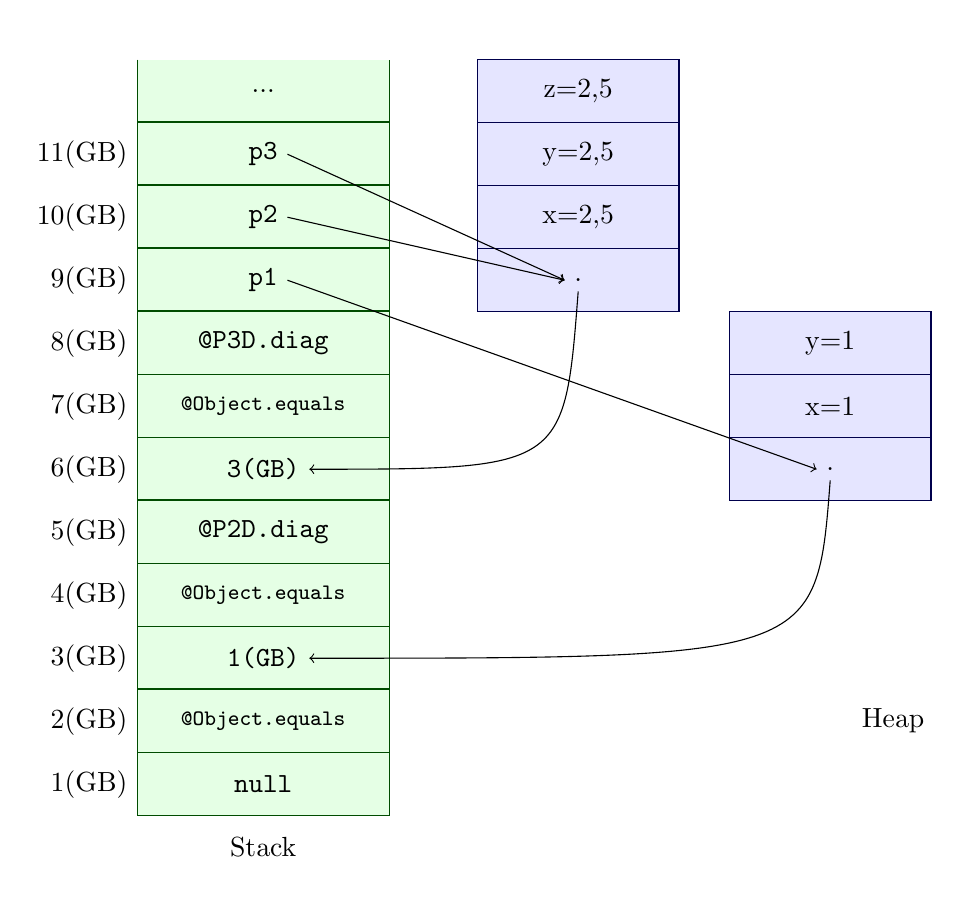
\begin{tikzpicture}[scale=.8]

	\stacktop{}
	\separator
	\cell{\texttt{p3}}        \cellcomL{11(GB)} \coordinate (p3) at (currentcell.east);
	\separator
	\cell{\texttt{p2}}        \cellcomL{10(GB)} \coordinate (p2) at (currentcell.east);
	\separator
	\cell{\texttt{p1}}        \cellcomL{ 9(GB)} \coordinate (p1) at (currentcell.east);
	\separator
	\cell{\texttt{@P3D.diag}} \cellcomL{ 8(GB)}
	\cell{\texttt{\footnotesize @Object.equals}} \cellcomL{ 7(GB)}
	\cell{\texttt{3(GB)}}     \cellcomL{ 6(GB)} \coordinate (T1) at (currentcell.east);
	\separator
	\cell{\texttt{@P2D.diag}} \cellcomL{ 5(GB)}
	\cell{\texttt{\footnotesize @Object.equals}} \cellcomL{ 4(GB)}
	\cell{\texttt{1(GB)}}     \cellcomL{ 3(GB)} \coordinate (T2) at (currentcell.east);
	\separator
	\cell{\texttt{\footnotesize @Object.equals}} \cellcomL{ 2(GB)}
	\cell{\texttt{null}}      \cellcomL{ 1(GB)}
	\cell[draw=none]{Stack}
	
	
	\drawstruct{(5,1)})
	\structcell{z=2,5}
	\structcell{y=2,5}
	\structcell{x=2,5}
	\structcell{.} \coordinate (O1) at (currentcell.west);
	\coordinate (O1l) at (currentcell.south);
	
	\drawstruct{(9,-3)}
	\structcell{y=1}
	\structcell{x=1}
	\structcell{.} \coordinate (O2) at (currentcell.west);
	\coordinate (O2l) at (currentcell.south);
	
	\draw[->] (p3) -- (O1);
	\draw[->] (p2) -- (O1);
	\draw[->] (p1) -- (O2);
	
	\draw[->] (O1l) .. controls (O1 |- T1) .. (T1);
	\draw[->] (O2l) .. controls (O2 |- T2) .. (T2);
	
	\draw (10,-10) node{Heap};

\end{tikzpicture}

\end{document}